\pagebreak
\newsection{Segnalazione errori}
Nel caso in cui dovessero essere riscontrati eventuali errori o criticità è possibile segnalarli attraverso l'indirizzo email del gruppo oppure aprendo una segnalazione nell'apposita sezione "\gl{Issue}" della repository in cui risiede il plug-in.

\subsection{Segnalazione con email}
L'indirizzo del gruppo è: {\url{7dos.swe@gmail.com}}. \\
Inserire nell'oggetto la segnatura "[BUG]" per segnalare che si tratta di un errore, seguita da una breve e concisa descrizione dello stesso.
Indicare nel corpo dell'email:
\begin{itemize}
	\item Versione di Grafana;
	\item Versione del plug-in;
	\item Browser e relativa versione;
	\item Sistema operativo e relativa versione;
	\item Descrizione dettagliata dell'errore.
\end{itemize}

\begin{figure} [H]
	\centering
	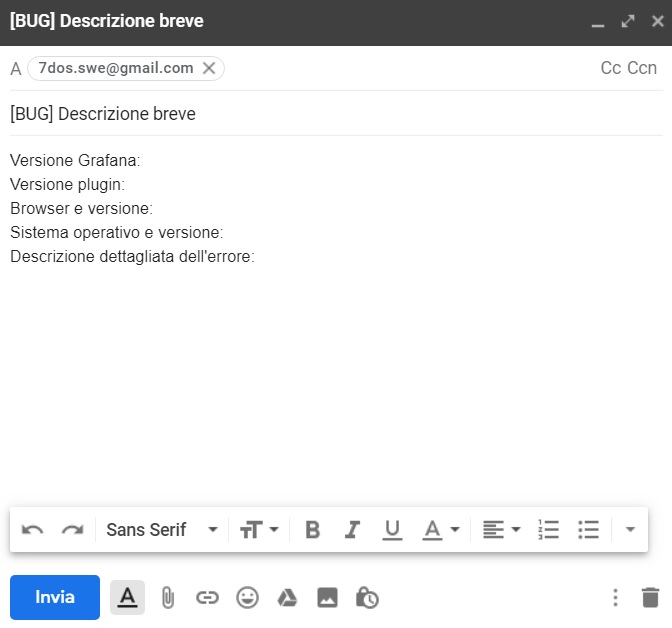
\includegraphics[scale=0.9]{Img/email.jpg} 
	\caption{Template email per segnalazioni} \label{} 
\end{figure} 

\subsection{Segnalazione su GitHub}

La repository del plug-in è: \url{https://github.com/NicoloTartaggia/7DOS-plugin}. \\
Posizionarsi nella sezione \emph{"Issues"} e premere il pulsante \emph{"New issue"}. Inserire nel titolo la segnatura "[BUG]" per segnalare che si tratta di un errore, seguita da una breve e concisa descrizione dello stesso.
Indicare nel corpo della \gl{issue}:
\begin{itemize}
	\item Versione di Grafana;
	\item Versione del plug-in;
	\item Browser e relativa versione;
	\item Sistema operativo e relativa versione;
	\item Descrizione dettagliata dell'errore.
\end{itemize}
\begin{figure} [H]
	\centering
	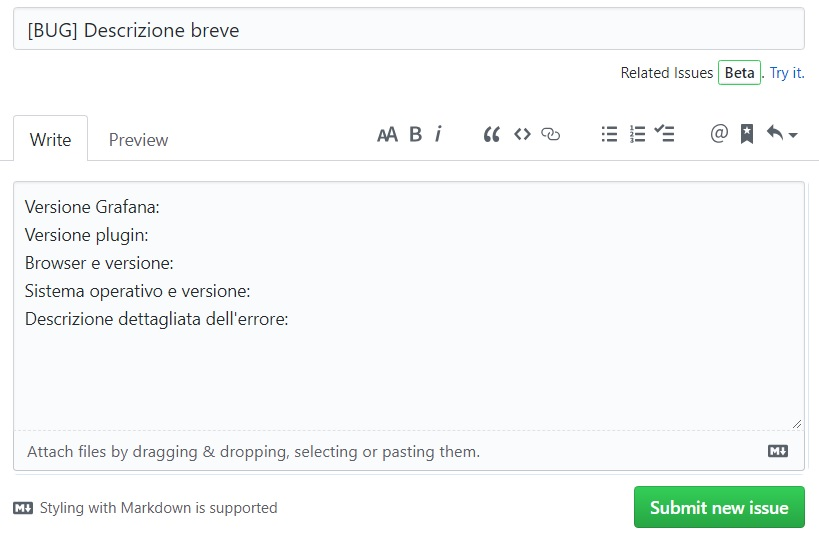
\includegraphics[scale=0.9]{Img/issue.jpg} 
	\caption{Template issue per segnalazioni} \label{} 
\end{figure} 

\newpage